\def\year{2015}
%File: formatting-instruction.tex
\documentclass[letterpaper]{article}
\usepackage{aaai}
\usepackage{times}
\usepackage{helvet}
\usepackage{courier}
\usepackage{graphicx}
\usepackage{tikz}
\usepackage[noend]{algpseudocode}
\usepackage{algorithm}
\usepackage{cleveref}
\usetikzlibrary{arrows,positioning,automata}
\frenchspacing
\setlength{\pdfpagewidth}{8.5in}
\setlength{\pdfpageheight}{11in}
\pdfinfo{
/Title (Insert Your Title Here)
/Author (Put All Your Authors Here, Separated by Commas)}
\setcounter{secnumdepth}{0}
 \begin{document}
% The file aaai.sty is the style file for AAAI Press 
% proceedings, working notes, and technical reports.
%
\title{Appraisal in Human-Robot Collaboration}
\author{Mahni Shayganfar, Charles Rich, Candace L. Sidner\\
Worcester Polytechnic Institute\\
Comoputer Science Department\\
100 Institute Road\\
Worcester, Massachusetts 01609\\
mshayganfar $|$ rich $|$ sidner @wpi.edu
}
\maketitle
\begin{abstract}
\begin{quote}
Don't know yet!\end{quote}
\end{abstract}

\section{Introduction}

- SharedPlans theory.

\noindent - Appraisal theory and social context.

\noindent - The necessity for identifying underlying processes of the
collaboration.

\section{Example Scenario}

Two short interactions of the robot and the astronaut (to be used throughout
the paper).

\section{Affective Motivational Collaboration Theory}
The Affective Motivational Collaboration Theory is built on the foundations of
the \textit{SharedPlans} theory of collaboration \cite{grosz:plans-discourse}
and the \textit{cognitive appraisal} theory of emotions
\cite{gratch:domain-independent}. Affective Motivational Collaboration Theory is
about the interpretation and prediction of observable behaviors in a dyadic
collaborative interaction. The theory focuses on the processes regulated by
emotional states. The observable behaviors represent the outcome of reactive and
deliberative processes related to the interpretation of the self's relationship
to the collaborative environment. Affective Motivational Collaboration Theory
aims to explain both rapid emotional reactions to events as well as slower, more
deliberative responses. The reactive and deliberative processes are triggered by
two types of events: \textit{external} events, such as the other's
\textit{utterances} and \textit{primitive actions}, and \textit{internal}
events, comprising changes in the self's mental states, such as belief formation
and emotional changes. Affective Motivational Collaboration Theory explains how
emotions regulate the underlying processes when these events occur during
collaboration. This theory elucidates the role of motives as goal-driven
emotion-regulated constructs with which an agent can form new intentions to cope
with internal and external events (cite my own AAAI paper).

Affective Motivational Collaboration Theory explains the functions of emotions
in a dyadic collaboration and show how affective mechanisms can coordinate
social interactions by enabling one to anticipate other's emotions, beliefs and
intentions. Our focus is on the mechanisms depicted as mental processes in
Figure \ref{fig:cpm} along with the mental states. The \textit{Mental States}
includes self's (robot's) beliefs, intentions, motives, goals and emotion
instances as well as the anticipated Mental States of the other (human). The
\textit{Collaboration} mechanism maintains constraints on actions, including
task states and the ordering of tasks. The \textit{Collaboration} mechanism also
provides processes to update and monitor the shared plan. The \textit{Appraisal}
mechanism is responsible for evaluating changes in the self's Mental States, the
anticipated Mental States of the other, and the state of the collaboration
environment. The \textit{Coping} mechanism provides the self with different
coping strategies associated with changes in the self's mental states with
respect to the state of the collaboration. The \textit{Motivation} mechanism
operates whenever the self a) requires a new motive to overcome an internal
impasse in an ongoing task, or b) wants to provide an external motive to the
other when the other faces a problem in a task. The \textit{Theory of Mind}
mechanism is the mechanism that infers a model of the other's anticipated mental
state. The self progressively updates this model during the collaboration.

\begin{figure}[tbh]
  \centering
  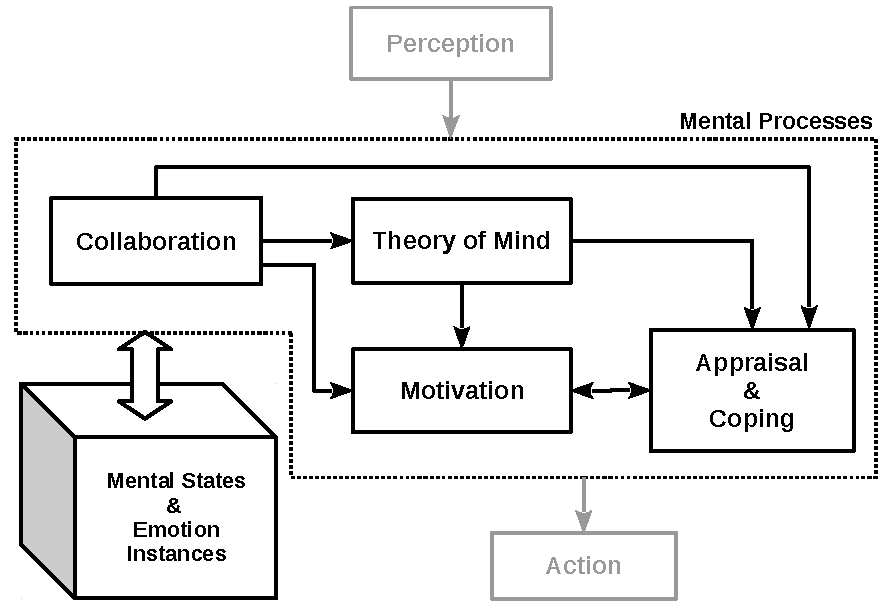
\includegraphics[width=0.474\textwidth]{figure/theory-general-croped.pdf}
  \caption{Computational framework based on Affective Motivational Collaboration
  Theory (arrows indicate primary influences between mechanisms).}
  \label{fig:cpm}
\end{figure}

\subsection{Mental States}
\label{sec:mental-states}

The Mental States shown in Figure \ref{fig:cpm} comprise the knowledge
base required for all the mechanisms in the overall model.

Mental states are conscious states of the mind providing the content for
cognitive processes. Affective Motivational Collaboration Theory operates with
the following Mental States: beliefs, intentions, motives, goals and emotion
instances. These Mental States possess attributes, each of which provides a
discriminating and unique interpretation of the related cognitive entities. The
self uses Mental States' attributes whenever there is an arbitration in the
internal cognitive processes. The Appraisal mechanism and the Motivation
mechanism play an essential role in computing the value of these attributes. I
provide more details about these attributes in this section.

\subsubsection{Belief:}

\textit{Beliefs} are a crucial part of the Mental States. I have two different
perspectives on categorization of beliefs. In one perspective, I categorize
beliefs based on whether they are shared or not between the collaborators. The
SharedPlans \cite{grosz:plans-discourse} theory is the foundation of this
categorization in which for any given proposition the agent may have: a) private
beliefs (the agent believes the human does not know these), b) the inferred
beliefs of the human (the agent believes the human collaborator has these
beliefs), and c) mutual beliefs (the agent believes both the self and the human
have these same beliefs and both of them believe that). From another
perspective, I categorize beliefs based on who or what they are about. In this
categorization, beliefs can be about the self, the other, or they can be about
the environment. Beliefs about the environment can be about internal events,
such as outcomes of a new appraisal or a new motivate, or external events such
as the human's offer, question or request, and general beliefs about the
environment in which the agent is situated. Beliefs can be created and updated
by different processes. They also affect how these processes function as time
passes.

The attributes of a belief are involved in arbitration procedures within
different processes in the \textit{Affective Motivational Collaboration Theory}.
They impact a range of these processes from, the formation of new beliefs, the
evaluation of an external event by the Appraisal mechanism, generation of new
motives, updates on collaboration plan, to the activation of coping strategies
and ultimately the self's behavior. The following six attributes of beliefs
are most related to \textit{Affective Motivational Collaboration Theory}.

\begin{itemize}
  \item \textbf{\textit{Strength:}} Belief strength is about how strong the self
  holds salient beliefs about an object, an entity, or an anticipated behavior.
  It can be measured through scales, for instance, how probable or likely that
  belief is, or just whether it is true or false. The strength of a belief can
  impact the self's intention attributes such as the \textit{certainty} or
  \textit{ambivalence}. A belief can be strong, but not accurate.
  
  \item \textbf{\textit{Accuracy:}} Accuracy of a belief is the relation between
  that belief and the truth which that belief is about. The accuracy of a belief
  can be measured by looking at how closely that belief can relate to the truth.
  The accuracy of a belief as a gradational property can be used in evaluative
  processes of the self, i.e., Appraisal. It can also impact the self's other
  goal-driven processes, e.g., Motivation, by updating the utility function(s)
  with respect to the estimated belief accuracy.
  
  \item \textbf{\textit{Frequency:}} The frequency of a belief is related to how
  regularly it appears as the result of an internal or an external event. The
  frequency of beliefs can impact attributes of the self's other Mental States.
  For instance, beliefs forming or maintaining intentions with direct
  experiences are more likely to occur frequently.
  
  \item \textbf{\textit{Recency:}} The recency of a belief refers to how
  temporally close a particular belief is to the current state of collaboration.
  The recency attribute of the self's belief can bias (recency effect) the
  evaluation processes of the cognitive mechanism during collaboration. It can
  create a tendency to weight recent events more than earlier ones whenever it
  is required according to self's Mental States. The self can allow or hinder
  this tendency to adopt an appropriate Coping mechanism.
  
  \item \textbf{\textit{Saliency:}} The saliency of a belief is a cognitive
  attribute that pertains to how easily the self becomes aware of a belief.
  This property of a belief has a prominent influence on the attention mechanism
  during collaboration. It directs the self's focus of attention to the most
  pertinent spatio-temporal salient internal or external event(s). Although
  belief saliency can determine the self's focus of attention, the self does not
  necessarily select an action based on the salient events.
  
  \item \textbf{\textit{Persistence:}} It is argued that beliefs form and change
  due to cognitive and social considerations \cite{carley:belief-persistence}.
  Persistent beliefs are very resistant to these changes. However, even
  persistent beliefs can change. Persistence of goal-related belief(s)
  influences the self's intentions and subsequently behaviors.
\end{itemize}

\subsubsection{Motive:}

\textit{Motives} are mental constructs which can initiate, direct and maintain
goal-directed behaviors. They are created by the emotion-regulated Motivation
mechanism. Motives can cause the formation of a new intention for the agent
according to: a) its own emotional states (how the agent feels about something),
b) its own private goal (how an action helps the agent to make progress), c) the
collaboration goal (how an action helps to achieve the shared goal), and d)
other's anticipated beliefs (how an action helps the other). Motives also
possess a set of attributes, e.g., \textit{Insistence} or \textit{Failure
Disruptiveness}. These attributes are involved in comparison of newly generated
motives based on the current state of the collaboration. Ultimately, the agent
forms or updates a belief about the winning motive in the Mental States.

According to Sloman, motives can be compared on various dimensions
\cite{sloman:motivation}. This comparison is based on motive attributes. In
\textit{Affective Motivational Collaboration Theory} motives are formed based on
the self's existing Mental States under the influence of Appraisal mechanism. The
existence of different Mental States, and the results of self appraisal as
well as the reverse appraisal of the other can cause a variety of motives to be
formed. The Motivation mechanism needs a set of attributes to compare newly
generated motives and choose the one which is most related to the current state
of the collaboration. I have chosen the following five motive attributes as
most related to the collaboration context.

\begin{itemize}
  \item \textbf{\textit{Insistence:}} The insistence of a motive defines the
  ``interrupt priority level'' of the motive, and how much that motive can
  attract the self's focus of attention. This dimension of motive is associated
  with what the Appraisal mechanism considers as \emph{relevance} and
  \emph{desirability} when evaluating an event. Beliefs about successive
  subgoals and the other's anticipated Mental States influence the insistence
  attribute of a motive. Insistent motives have higher priority and are able to
  interrupt self's ongoing tasks. The insistence of a motive is a function of
  the importance, urgency and the elapsed time for that motive.
  
  \item \textbf{\textit{Importance:}} The importance of a motive is determined
  by the corresponding beliefs about the effects of achieving or not achieving
  the associated goal. It is a function of belief attributes (including
  strength, accuracy, frequency, recency, saliency and persistence) and the
  current goal. For instance, if a motive is supported by a belief about the
  current goal with relatively high attribute values, that motive will become
  important for the self.
  
  \item \textbf{\textit{Urgency:}} The urgency of a motive defines how much time
  the self has to acknowledge and address that motive before it is too late.
  The urgency of a motive is a function of beliefs about the other's mental
  states as well as the required and the estimated time to fulfill the
  associated goal. For instance, the self responds to an urgent motive due to
  the existence of an important anticipated outcome for the other, and limited
  time to accomplish the corresponding tasks, even if those tasks are not
  important for the self.
  
  \item \textbf{\textit{Intensity:}} The intensity of a motive determines how
  actively and vigorously that motive can help the self to pursue the goal if
  adopted. Motives with higher intensity will motivate the self to apply
  certain types of coping processes for an obstructed goal to avoid termination
  of the collaboration. Motives with higher intensity cause the self to find
  alternative solutions for the problem rather than abandoning the goal and
  ultimately the collaboration.
  
  \item \textbf{\textit{Failure Disruptiveness:}} The failure disruptiveness
  attribute of a motive determines how disruptive failure is to achieving the
  corresponding goal. In other words, it gives the self a measure of the
  pleasantness of achieving a related goal. This attribute directs the self's
  behavior toward positive and negative outcomes during collaboration. It also
  plays a role in performance assessment processes when the self needs to
  compare its competence level on a given task relative to the other.
\end{itemize}

\subsubsection{Intention:}

\textit{Intentions} are mental constructs directed at future actions. They play
an essential role in: a) taking actions according to the collaboration plan, b)
coordination of actions with human collaborator, c) formation of beliefs about
self and anticipated beliefs about the other, and d) behavior selection in the
Coping mechanism. First, taking actions means that the agent will intend to take
an action for primitive tasks that have gained the focus of attention, possess
active motives, have satisfied preconditions for which required temporal
predecessors have been successfully achieved. Second, intentions are involved
in action coordinations in which the human's behavior guides the agent to infer
an anticipated behavior of the human. Third, intentions play a role in belief
formation mainly as a result of the permanence and commitment inherent to
intentions in subsequent processes, e.g., appraisal of the human's reaction to
the current action and self regulation. And lastly, intentions are involved in
selecting intention-related strategies, e.g., planning, seeking instrumental
support and procrastination, which these strategies are an essential category of
the strategies in the Coping mechanism. Intentions possess a set of attributes,
e.g. \textit{Involvement, Certainty, Ambivalence} which moderate the consistency
between intention and behavior. The issue of consistency between the intentions
(in collaboration) and the behaviors (as a result of the Coping mechanism in the
appraisal cycle) is important because neither of these two mechanisms alone
provides solution for this concern.

The attributes of an intention influence several processes in \textit{Affective
Motivational Collaboration Theory}. They are involved in mechanisms such as
Appraisal and Motivation as well as other Mental States, e.g., goals. One of the
most important uses of intention attributes is to moderate the
intention-behavior relations \cite{cooke:intention-behavior-consistency}.
Ultimately, the self can show more consistent behavior with respect to its own
preceding behaviors and current state of the collaboration. I decided to include
the following five intention attributes extracted from the psychology literature
in \textit{Affective Motivational Collaboration Theory}.

\begin{itemize}
  \item \textbf{\textit{Temporal Status:}} The temporal status of an intention
  can be defined as the extent to which an intention remains consistent over
  time. The self needs to maintain the stability of its intentions as time
  passes until the task is performed. Temporally stable intentions helps the
  other to accurately predict the self's behavior. The anticipated cognitive
  load of perceiving the self's task by the other impacts the temporal stability
  of the self's intention. In other words, the temporal stability of an
  intention moderates the intention-behavior relation of the self during
  collaboration.
  
  \item \textbf{\textit{Direct Experience:}} The direct experience of an
  intention refers to whether the self previously has performed a task based on
  the similar intention. The self can refer to the corresponding Mental States
  of the intention directly experienced in the past before taking a new action.
  The Mental States associated with the prior experience of an intention can
  influence the appraisal of a new event requiring the self to perform the same
  task. For instance, the existence of a direct experience of an intention
  impacts the degree of the \textit{expectedness} and \textit{controllability}
  of an event during the collaboration which ultimately guides the Coping
  mechanism to produce an appropriate behavior.
  
  \item \textbf{\textit{Certainty:}} The certainty of an intention is determined
  by the quality of the underlying motive and the beliefs associated with that
  motive. The more \textit{strong, accurate, frequent, recent, salient} and
  \textit{persistent} a set of pertinent beliefs of the self are, the more
  chance the related motive has to be selected. Since the certainty of an
  intention depends on the associated motive, the nature of the pursued goal also
  implicitly impacts the certainty of that intention. A goal with higher
  \textit{specificity} value influences the Belief Formation process of a new
  motive by increasing the certainty of the affiliated intention. The certainty
  of an intention is an important moderator of the self's intention-behavior
  consistency.
  
  \item \textbf{\textit{Ambivalence:}} The Mental States of the self might
  contain contradictory intentions towards the pursuit of the same goal, which
  makes those intentions ambivalent. For instance, the self might already have
  an intention to perform a task according to the shared plan, while the Appraisal
  and the Motivation mechanisms dynamically provide a new motive forming a new
  opposing intention. Furthermore, ambivalent intentions can occur because of
  the contrast between the self's private goal and the shared goal during the
  collaboration. The ambivalence attribute of an intention is against the
  intention-behavior consistency of the self.
  
  \item \textbf{\textit{Affective-Deliberative Consistency:}} The self's
  intentions possess an affective and a deliberative component. The affective
  component refers to the emotion instance and in general the affective
  evaluation of the self's intention towards its own behavior. However, the
  deliberate component refers to the self's actual intention which is formed
  either based on the existing shared plan or through a new motive generated by
  the Motivation mechanism. For instance, as an example of
  affective-deliberative inconsistency, the self can appraise the formation of
  the current intention as an \textit{urgent} and \textit{uncontrollable} one
  (which leads the self's emotion towards anger), despite the fact that
  performing the task associated with this intention is required for the
  satisfaction of the shared plan. In general, mutually consistent affective and
  deliberate components of an intention positively impacts the consistency of
  the self's intention and behavior.
\end{itemize}

\subsubsection{Goal:}

\textit{Goals} help the agent to create and update its collaboration plan
according to the current private and shared goal content and structure, i.e.,
the \textit{Specificity, Proximity} and \textit{Difficulty} of the goal. Goals
direct the formation of intentions to take appropriate corresponding actions
during collaboration. Goals also drive the Motivation mechanism to generate
required motive(s) in uncertain or ambiguous situations, e.g., to minimize the
risk of impasse or to reprioritize goals. The \textit{Specificity} of goals has
two functions for the agent. First, it defines the performance standard for
evaluating the progress and quality of the collaboration. Second, it serves the
agent to infer the winner of competing motives. The \textit{Proximity} of goals
distinguishes goals according to how ``far'' they are from the ongoing task.
Proximal (or short-term) goals are achievable more quickly, and result in higher
motivation and better self-regulation than more temporally distant (or
long-term) goals. Goals can influence the \textit{Strength} of beliefs, which is
an important attribute for regulating the elicitation of social emotions. The
\textit{Difficulty} of goals impacts collaborative events and decisions in the
appraisal, reverse appraisal, motive generation and intention formation
processes. For instance, overly easy goals do not motivate; neither are people
motivated to attempt what they believe are impossible goals.

The attributes of a goal also impact the processes in \textit{Affective
Motivational Collaboration Theory}, especially the processes involved in
Motivation and Appraisal mechanisms. The attributes of a goal are important
because the Motivation and the Appraisal mechanisms in this theory are
goal-driven and attribution of the goals according to the self's standards
provides coherency of the processes and their outcomes. I discuss the three most
relevant goal attributes in this section.

\begin{itemize}
  \item \textbf{\textit{Proximity:}} Goals can be distinguished by how far they
  project into the future during the collaboration. Proximal (short-term) goals
  result in more related motives and subsequently better self and
  social-regulation than temporally distant goals. Proximal goals impact the
  self's behaviors by influencing the evaluation process of the Appraisal
  mechanism. As a result, the self can determine the collaboration progress
  towards the shared goal more accurately while operating based on proximal
  goals.
  
  \item \textbf{\textit{Specificity:}} Goals incorporating specific performance
  standards are more likely to enhance the self's self-evaluation than general
  goals. Specific goals raise the self-evaluation performance because they
  provide a more accurate baseline for the mechanisms, e.g., Appraisal or
  Motivation, that the self needs for self-evaluation during collaboration.
  Consequently, by increasing the self-evaluation performance, the self can
  compute more accurate anticipated self-satisfaction. For instance, holding an
  object A in a particular position with respect to an object B for a certain
  amount of time and welding them with a material C is a more specific goal than
  a general goal of installing an object A on object B.
  
  \item \textbf{\textit{Difficulty:}} The goals that are moderately difficult
  have the most impact on the Motivation mechanism, and ultimately the self and
  social regulation processes of the self. Conversely, overly easy or impossible
  goals usually do not motivate an individual to achieve the goal. Difficult
  goals increase the probability of a motive's \textit{failure disruptiveness},
  and overly easy goals decrease the \textit{importance} of the related motive;
  in both cases the motives have less chances to form new intentions. The lower
  chance of new intention formation will disrupt the self and social regulation
  since the self cannot regulate internal processes and influence the external
  world without forming appropriate intentions to take required actions. The
  existence of a partial shared plan, dependency on the other to perform a task,
  the failure of the same or similar task in the past and the conflict between
  the self's private goal and the shared goal all increase the difficulty level
  of a goal.
\end{itemize}

\subsubsection{Emotion Instance:}

\textit{Emotions} in Mental States are emotion instances that are elicited by
the Appraisal mechanism for list of emotion types used in this model). The agent
also keeps beliefs about these emotion instances in the Mental States. The
Belief Formation mechanism creates or updates these beliefs about emotions.
These emotion instances include the agent's own emotions as well as the
anticipated emotions of the other which are created with the help of the
processes in the Theory of Mind mechanism.

Each emotion has its own functionality in either intrapersonal or interpersonal
level. These emotions not only regulate the self's internal processes, but also
assist the self to anticipate the other's Mental States. In this section, I
provide the description of some of the emotions that can be elicited during
collaboration, and are involved in our scenario. In this document, to avoid
controversial issue of whether virtual agents or robots can feel emotions, I am
going to use the convention of having emotions by the agent or the robot. The
agent can also possess belief about an emotion instance which is similar to
having belief about any other proposition.

\begin{itemize}
  \item \textbf{\textit{Joy:}} Joy is the state of an individual's well-being
  and is associated with the sense of successful achievement of a goal. Joy
  reveals one's sense of pleasure which implies an impending gain for the
  individual.
  
  \item \textbf{\textit{Anger:}} Anger can be elicited by an unfair obstacle,
  hindering the individual's goal attainment and it is usually triggered by some
  external event (e.g., threat) which provokes a behavioral reaction. Anger
  functions to set boundaries or escape from dangerous situations, and implies
  an urgent desire for justice.
  
  \item \textbf{\textit{Hope:}} Hope is the result of an optimistic evaluation
  of an event by an individual having expectations of positive and desirable
  future outcomes related to that event. It is usually a poignant assimilation
  of the present discontent and the future content implying an imagined or
  anticipated successful future goal state.
  
  \item \textbf{\textit{Guilt:}} Guilt is based on self-condemnation in response
  to a negative outcome of one's self performance evaluation. It is caused by
  the violation of others' beliefs about the self, and others' standards and
  bearing significant responsibility due to that violation. The occurrence of
  guilt usually implies the desire to atone in social context.
  
  \item \textbf{\textit{Pride:}} Pride is a product of the satisfied sense of
  one's own actions or decision outcomes. It implies the self-approval of the
  evaluation oucomes of one's own actions. Pride is associated with the
  achievement motivation wherein succeeding at a particular goal motivates the
  corresponding action.
  
  \item \textbf{\textit{Shame:}} Shame is produced when one evaluates one's own
  actions or behaviors and attributes failure to the outcome. The individual
  focuses on specific features of self which led to failure. Shame implies the
  existence of remorse.
  
  \item \textbf{\textit{Worry:}} Worry is one's emotional attempt to avoid
  anticipated potential threats or unidentified undesirable events. The
  individual's concern can be about a real or an imagined issue. Worry implies a
  fear of a future failure about which one should make a decision or take an
  action at present.
\end{itemize}

\subsection{Collaboration Mechanism}

Short paragraph to describe collaboration mechanism and its role in overall
system (mention that we are not talking about the algorithms in this mechanism).

Then, describe the collaboration model and its components.

The Collaboration mechanism is responsible for maintaining the internal
structure of a collaboration, including the focus of attention, constraints on
actions, updating the shared plan and, in general, monitoring of the
collaboration. All of these structures require updating each time the self
receives an external event. For instance, an utterance by the other can impact
the self's focus of attention during the collaboration, or the effect of a
primitive action can influence the self's view of an impasse on a task. As
another example, the perception of the other's emotion instance can cause
significant changes in the self's collaboration monitoring. The Collaboration
mechanism also responds to internal events. These changes can occur under the
influence of several other processes which are able to alter the self's mental
states. For instance, the Motivation mechanism can generate a new motive which
causes the self to add a new intention to its own Mental States.

\begin{itemize}
  \item \textbf{Input:} The input to the \textit{Collaboration} mechanism
  includes all the data that affects the execution of individual tasks in the
  collaboration plan. This data will be provided via the different elements of
  Mental States including beliefs, intentions and goals. These Mental States
  will establish agent's initial plan and will be updated throughout the
  collaboration process by the Perception and Inference mechanisms.
  
  \item \textbf{Output:} The output of \textit{Collaboration} includes all the
  data that is modified or created during execution of a plan in the form of
  Mental States. These Mental States will be used by the internal processes in
  the Theory of Mind mechanism. Additionally, the Appraisal mechanism will use
  these Mental States to evaluate the events during collaboration. These Mental
  States also will be used by the Inference mechanism for the purpose of
  maintaining the collaboration.
  
  \item \textbf{Function:} The \textit{Collaboration} mechanism will construct a
  hierarchy of tasks and also manage and maintain the constraints and other
  required details of the collaboration specified by the plan. These details
  include the inputs and outputs of individual tasks, the \textit{preconditions}
  specifying whether it is appropriate to perform a task, and the
  \textit{postconditions} specifying whether a just-completed task was
  successful (which can be used as an indication of an impasse or failure).
  \textit{Collaboration} also keeps track of the focus of attention, which
  determines the salient objects, properties and relations at each point of the
  collaboration. Moreover, \textit{Collaboration} has the ability to shift the
  focus of attention during the collaboration. All the other mechanisms in the
  overall \textit{Affective Motivational Collaboration Model} are influenced by
  changes in the collaboration plan.
\end{itemize}

\subsection{Appraisal Mechanism}

\subsection{Appraisal of External Events}

The other's \textit{utterances}, the effect(s) of the collaborators'
\textit{primitive actions}, and the other's \textit{emotion instances}
(expressed nonverbally) are the three types of external events perceived by the
self during collaboration. The Appraisal mechanism receives the output of the
Perception and Collaboration mechanisms as well as the requisite Mental States
related to current event. It appraises the external event, in terms of appraisal
variables using, a) the collaboration structure, b) the social characteristics
of collaboration, and c) the history of the self's related Mental States. The
collaboration structure contains information about the collaboration's shared
plan and the collaborators' shared goal, the temporal and the hierarchical
constraints of the tasks, and the current focus of attention. 

The social characteristics of collaboration (see Section are conceptual
properties associated with collaboration. These concepts provide deeper
understanding of the collaborative interactions in terms of the underlying
processes from both the personal and the social perspectives. Furthermore, these
concepts determine when each process is used during a collaboration and why.
Lastly, the self will progressively generate and update various types of Mental
States during collaboration. The occurrence of a new external event causes a
change in the self's Mental States. The construct of the new mental state, e.g.,
beliefs, are semantically connected to the older ones. The Appraisal mechanism
uses the history of the Mental States to consistently evaluate a new external
event.

\subsection{Appraisal of Internal Events}

The formation of a \textit{new belief} (one that has not already been evaluated
by the Appraisal mechanism, such as a belief about a new motive), and the
formation of a \textit{new motive}, are the two types of internal events that
will be evaluated by the Appraisal mechanism. Thus, the Appraisal mechanism is
involved in the formation of a new belief to ultimately create balanced
behaviors during the course of a collaboration. The Appraisal mechanism receives
the output of the Theory of Mind and Motivation mechanisms as well as the
available Mental States (e.g., beliefs about the current emotion instances of
the self and the other) and evaluates the environment in terms of the appraisal
variables whenever a new belief is generated. As mentioned in Section, a) the
collaboration structure, b) the social characteristic of the collaboration, and
c) the history of the self's Mental States, are also crucial in the evaluation
of internal events. The outcome of this appraisal process can result in a new
belief about emotion instances, e.g. believing to have hope, or it can generate
beliefs about different attributes of the Mental States of the self or the
other.

\subsection{Appraisal}

\begin{itemize}
  \item \textbf{Input:} The most significant part of \textit{Appraisal's} input
  data is based on the activity of the Collaboration mechanism. This data
  includes all the required Mental States associated with the Collaboration
  mechanism. For instance, the beliefs and their Strengths will be used by
  algorithms inside of \textit{Appraisal} to compute the value of the appraisal
  variables. \textit{Appraisal} also receives data from the Theory of Mind
  mechanism. This data helps the agent use \textit{Appraisal} for inferring
  the human's intentions and motives based on a reverse appraisal procedure.
  
  The input data from the Perception is generally needed to support the
  evaluation of the events. The Motivation mechanism sends data to
  \textit{Appraisal} whenever, for example, a new set of motives is being
  generated or the motive comparator wants to evaluate different motives for an
  arbitration procedure.
   
  \item \textbf{Output:} The output of \textit{Appraisal} can directly and
  indirectly impact other mechanisms. The Motivation mechanism uses this data to
  generate, compare and monitor motives based on the current internal appraisal
  of the agent as well as the appraisal of the environment. This output data
  also assists the Belief Formation mechanism to create new beliefs about the
  current emotional state of the agent or the human as well as the corresponding
  appraisal of individual motives.
  
  \item \textbf{Function:} \textit{Appraisal} is a subjective evaluation
  mechanism based on individual processes each of which computes the value of
  the appraisal variables used in my computational model. The Collaboration
  mechanism needs the evaluative assistance of the \textit{Appraisal} mechanism
  for various reasons. The course of a collaboration is based on a full or a
  partial plan which needs to be updated as time passes and collaborators
  achieve, fail at or abandon a task assigned to them. The failure of a task
  should not destroy the entire collaboration. Appraising the environment and
  the current events helps the agent to update the collaboration plan and avoid
  further critical failures during collaboration. \textit{Appraisal} also helps
  the agent to have a better understanding of the human's behavior by making
  inferences based on appraisal variables. Furthermore, in order to collaborate
  successfully, a collaborator cannot simply use the plan and reach to the
  shared goal; there should be an adaptation mechanism not only for updating the
  plan but also the underlying Mental States. For instance, there are beliefs
  about the appraisal of the self and the other that augment the model of what
  collaborators have done, and what and how they are planning to achieve the
  current shared goal based on their emotional states. This process will be
  discussed in more detail under the Motivation mechanism. Additionally, the
  beliefs formed based on the appraisals can impact other mechanisms such as the
  Theory of Mind, Motivation and Coping, essentially including the whole
  computational model.
  
\end{itemize}

\section{Mental Graph}
\label{sec:mental-graph}

A graph illustration of mental state and a clear short and desciptive
walkthrough example.

The \textit{F{\fontsize{8}{8}\selectfont IND}P{\fontsize{8}{8}\selectfont ATH}}
function uses the Dijkstra algorithm to find the shortest path.

\begin{center}
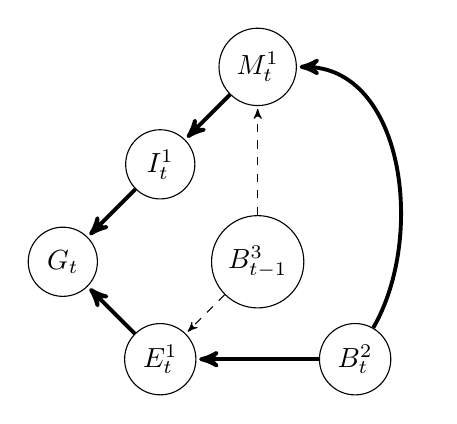
\begin{tikzpicture}[>=stealth',shorten >=1pt,node distance=1.75cm,on
grid,initial/.style    ={}] 
  \node[state]          (G)                         {$G_t$};
  \node[state]          (I1) [above right =of G]    {$I^1_t$};
  \node[state]          (E1) [below right =of G]    {$E^1_t$};
  \node[state]          (M1) [above right =of I1]   {$M^1_t$};
  \node[state]          (B1) [below right =of I1]   {$B^3_{t-1}$};
  \node[state]          (B2) [below right =of B1]   {$B^2_t$};
\tikzset{mystyle/.style={->,double=black}} 
\tikzset{every node/.style={fill=black}} 
\path (M1)    edge [mystyle]   (I1) 
      (B2)    edge [mystyle]   (E1)
      (I1)    edge [mystyle]   (G)
      (E1)    edge [mystyle]   (G);
\tikzset{mystyle/.style={->,dashed=black}}
\path (B1)    edge [mystyle]   (E1) 
      (B1)    edge [mystyle]   (M1);
\tikzset{mystyle/.style={->,relative=false,in=0,out=60,double=black}}
\path (B2)    edge [mystyle]   (M1); 
\end{tikzpicture}
\end{center}

\section{Appraisal Processes}

All of the algorithms use a mental graph which is a directed acyclic graph
constructed based on the mental states of the robot at each turn during the
collaboration (see Section \ref{sec:mental-graph}). They also use the
content of the most recent event at each turn which includes the associated
goal and the belief about the event. The associated goals can be any type
action, utterance, or emotional expression.

We found four appraisal variables, i.e., \textit{Relevance} (Algorithm
\ref{alg:relevance}), \textit{Desirability} (Algorithm \ref{alg:desirability}),
\textit{Expectedness} (Algorithm \ref{alg:expectedness}), and
\textit{Controllability} (Algorithm \ref{alg:controllability}) to be more
important than the other appraisal variables in a collaboration context.
There are other appraisal variables introduced in psychological
\cite{scherer:appraisal-processes} and computational literature
\cite{gratch:domain-independent}; we do not provide algorithms for them in this
paper. The concept behind these variables are either too simple, e.g.,
\textit{Perspective} (i.e., the view point from which an event is judged), or it
requires a particular approach which is not our concern in this paper, e.g.,
\textit{Likelihood} (i.e., how probable is the outcome of an event).

The \textit{recognizeGoal()} function returns the unique goal to which the event
directly contributes irrespective of the event type (i.e., action, utterance, or
emotional expression). This event structure holds in all of our algorithms.

\subsection{Relevance}

Relevance as an appraisal variable measures the significance of an event for the
robot. Relevance is an important appraisal variable since the other appraisal
dimensions are only derived for the relevant events.

Algorithm \ref{alg:relevance} determines the relevance of the given event with
respect to the shared goal. An event is \textit{irrelevant} if there is no
connection between the event and the current shared goal. If there is a
connection, the relevance of the event will depend on the significance of the
event with respect to the current collaboration status. The significance of an
event is determined based on the utility of the event as it is also presented in
\cite{gratch:domain-independent,marsella:ema-process-model}. We believe although
the utility of the event represents the sigificance of the event, the other
collaborator's expressed emotion also plays a role by influencing the
significance of the utility through a threshold. 

The algorithm starts by taking the belief about the current event
($\mathit{b}_{\varepsilon_t}$) and the shared goal associated with the current
mental graph ($g_{t}$). After perceiving an event, it is the belief about that
event which represents the event in robot's mental state. Continuing in line 3,
the $g_{t}$ represents the shared goal (in the mental graph) at time (turn) $t$
within the shared plan. Then, we find the shortest path ($\mathcal{P}_{t}$)
between the corresponding nodes of $\mathit{b}_{\varepsilon_t}$ and $g_{t}$ in
the mental graph. As we mentioned earlier, if there is no path between the
belief about the current event and the active shared goal, the algorithm finds
the event \textit{irrelevent} to the current shared goal, and terminates.
However, if there is a path between $\mathit{b}_{\varepsilon_t}$ and $g_{t}$, we
need a way to determine whether the event is relevant to the current
collaboration status. Thus, we compute the utility of an event and make our
decision with respect to the human's emotional state. In other words, the
relevance of a belief about an event is influenced by the perceived emotion of
the human collaborator. 

In line 8, the \textit{G{\fontsize{8}{8}\selectfont
ET}E{\fontsize{8}{8}\selectfont VENT}U{\fontsize{8}{8}\selectfont TILITY}}
function computes the utility of the event $\mathcal{U}$ such that ($0 \leq
\mathcal{U} \leq 1$) based on the values of the attributes associated with the
belief about that event, i.e., $\mathit{b}_{\varepsilon_t}$. And, the human's
emotion influences the decision about the utility of the event in form of a
threshold value ($\tau_{t}$). For instance, a positive expressed emotion of the
human reduces the threshold value which consequently makes the robot see an
event with even a slightly positive utility as a relevant one. Finally, if
$\mathcal{U}$ is greater than or equal to $\tau_{t}$ the event will be
considered \textit{relevant}; otherwise the event will be considered
\textit{irrelevant} even though there is a path between
$\mathit{b}_{\varepsilon_t}$ and $g_{t}$.

\begin{algorithm}
	\caption{(Relevance)}
	\label{alg:relevance}
	\begin{algorithmic}[1]
		\Function{IsEventRelevant}{{\fontsize{8.5}{9}\selectfont MentalGraph}
		$\mathcal{G}_{t}$, {\fontsize{8.5}{9}\selectfont Event} $\varepsilon_t$}
			\Statex
			\State $\mathit{b}_{\varepsilon_t} \gets \Call{getBelief}{\varepsilon_t}$
			\State $\mathit{g}_{t} \gets \textit{currGoal}{(\mathcal{G}_{t})}$
			\Statex
			\State $\mathcal{P} \gets \Call{findPath}{\mathit{b}_{\varepsilon_t},
			\mathit{g}_{t}}$
			\Statex
			\If {$(\mathcal{P} = \emptyset)$}
				\State \Return {{\fontsize{8}{8}\selectfont IRRELEVANT}}
			\Else
				\State $\mathcal{U} \gets \Call{getEventUtility}{\mathit{b}_{\varepsilon_t},
				\mathit{g}_{t}}$ 
				\State $\tau_{t} \gets \Call{getEmotionalThreshold}{\mathcal{G}_{t}}$
				\If {$( \mathcal{U} \geq \tau_{t} )$}
				\State \Return {{\fontsize{8}{8}\selectfont RELEVANT}}
				\Else
					\State \Return {{\fontsize{8}{8}\selectfont IRRELEVANT}}
				\EndIf
			\EndIf
		\EndFunction
	\end{algorithmic}
\end{algorithm}

\subsection{Desirability}

Desirability characterizes the value of an event to the robot in terms of
whether the event facilitates or thwarts the collaboration goal. Desirability
captures the valence of an event with repect to the robot's preferences
\cite{gratch:domain-independent}. In a collaborative robot preferences are
biased towards those events facilitating progress in the collaboration. An event
is desirable if it somehow facilitates the state of the shared goal, or if it
inhibits the state of a goal that is incosistent with respect to the shared
goal.

Desirability plays an important role in the overall architecture; it makes the
processes involved in the other mechanisms (e.g., Motivation or Theory of Mind)
and consequently the robot's mental state congruent with the collaboration
status which is the robot's desire. Therefore, it causes the robot to dismiss
events causing inconsistencies in the robot's collaborative behavior. Moreover,
desirability is also crucial from the collaboration's point of view. A
collaborative robot needs to know whether its own and the other collaborator's
actions, utterances, and emotional expressions are desirable in terms of their
consistence with the status of the current shared goal. In other words, the
collaboration mechanism uses the appraisal process of desirability to coordinate
what the self or the other does, says, and expresses during collaboration.
Reciprocally, the appraisal mechanism and in this case the desirability process
use the collaboration structure to obtain their required information.

Algorithm \ref{alg:desirability} provides a process in which the desirability of
an event is computed with regard to the status of the shared goal; i.e., it
operates based on whether and how the event changes the status of the current
shared goal. It receives the current mental graph, $\mathcal{G}_{t}$, and the
current event, $\varepsilon_t$, from input, and decides whether and how the
event is desirable or undesirable. First, the algorithm checks the status of the
collaboration's top level goal (lines 2 to 6), and if the the top level goal is
still in progress, it continues by checking the status of the current shared
goal (lines 7 to 13). If any of the top level and current shared goals are
achieved in these two steps, the robot interprets the event as a desirable one.
However, if any of these goals are blocked, the event will be considered
undesirable by the robot. 

The algorithm continues in the case of an unknown status of the current shared
goal, and checks whether the precondition(s) of the associated goal with the
current event, $\mathit{g}_{\varepsilon_t}$, are satisfied (lines 17 to 21).
Intuitively, the robot prefers the satisfied perconditions and interprets the
event as desirable while unsatisfied preconditions are undesirable for the
robot. For instance, a satisfied precondition of a future goal is still
desirable for the robot to some extent. Note that the robot also checks the
ambiguity of the associated goal with the current event (line 15). An ambiguous
goal is a goal which is not recognized in the robot's plan, and it is
undesirable for the robot. Afterall, if the preconditions of the associated goal
with the current event are unknown, the robot checks whether this goal,
$\mathit{g}_{\varepsilon_t}$, contributes to the current shared goal,
$\mathit{g}_{t}$ (lines 22 to 25). As a result a contributing goal will obtain a
neutral desirability in comparison with a noncontributing goal which will be
undesirable for the robot.

\begin{algorithm}
	\caption{(Desirability)}
	\label{alg:desirability}
	\begin{algorithmic}[1]
		\Function{IsEventDesirable}{{\fontsize{8.5}{9}\selectfont MentalGraph} 
		$\mathcal{G}_{t}$, {\fontsize{8.5}{9}\selectfont Event $\varepsilon_t$}}
			\Statex
			\If {(\textit{topLevelGoalStatus()} = {\fontsize{8}{8}\selectfont ACHIEVED})}
				\State \Return {{\fontsize{8}{8}\selectfont HIGHEST-DESIRABLE}}
			\ElsIf {(\textit{topLevelGoalStatus()} = {\fontsize{8}{8}\selectfont
			BLOCKED})} \State \Return {{\fontsize{8}{8}\selectfont HIGHEST-UNDESIRABLE}}
			\ElsIf {(\textit{topLevelGoalStatus()} = {\fontsize{7.4}{8}\selectfont
			INPROGRESS})}
				\Statex
				\If {(\textit{curGoalStatus()} = {\fontsize{8}{8}\selectfont ACHIEVED})}
					\State \Return {{\fontsize{8}{8}\selectfont HIGH-DESIRABLE}}
				\ElsIf {(\textit{curGoalStatus()} = {\fontsize{8}{8}\selectfont BLOCKED})}
					\State \Return {{\fontsize{8}{8}\selectfont HIGH-UNDESIRABLE}}
				\ElsIf {(\textit{curGoalStatus()} = {\fontsize{8}{8}\selectfont
				INPROGRESS})}
					\State \Return {{\fontsize{8}{8}\selectfont MEDIUM-DESIRABLE}}
				\ElsIf {(\textit{curGoalStatus()} = {\fontsize{8}{8}\selectfont UNKNOWN})}
					\Statex
					\State $\mathit{g}_{\varepsilon_t} \gets
					\textit{recognizeGoal}{(\varepsilon_t)}$
					\Statex
					\If {$(\mathit{g}_{\varepsilon_t} =$ {\fontsize{8}{8}\selectfont
						AMBIGUOUS}$)$}
						\State \Return {\fontsize{8}{8}\selectfont HIGH-UNDESIRABLE}
					\EndIf
					\Statex
					\If {(\textit{precondStatus($\mathit{g}_{\varepsilon_t}$)} =
					{\fontsize{8}{8}\selectfont SATISFIED})}
						\State \Return {{\fontsize{8}{8}\selectfont LOW-DESIRABLE}}
					\ElsIf {(\textit{{\fontsize{9}{9}\selectfont
					precondStatus($\mathit{g}_{\varepsilon_t}$)}} =
					{\fontsize{7}{8}\selectfont UNSATISFIED})} 
						\State \Return {{\fontsize{8}{8}\selectfont LOW-UNDESIRABLE}}
					\ElsIf {(\textit{precondStatus($\mathit{g}_{\varepsilon_t}$)} =
					{\fontsize{7}{8}\selectfont UNKNOWN})}
						\Statex
						\State $\mathit{g}_{t} \gets \textit{currGoal}{(\mathcal{G}_{t})}$
						\Statex
						\If {$(\textit{doesContribute}(\mathit{g}_{\varepsilon_t},
						\mathit{g}_{t}))$} 
							\State \Return {{\fontsize{8}{8}\selectfont NEUTRAL}}
						\ElsIf {$(\neg
						\textit{doesContribute}(\mathit{g}_{\varepsilon_t},\mathit{g}_{t})$}
							\State \Return {{\fontsize{8}{8}\selectfont MEDIUM-UNDESIRABLE}}
						\EndIf
					\EndIf
				\EndIf
			\EndIf
		\EndFunction
	\end{algorithmic}
\end{algorithm}

\subsection{Expectedness}

Expectedness is the extent to which the truth value of a state could have been
predicted from causal interpretation of an event
\cite{marsella:ema-process-model}. In the collaboration context the expectedness
of an event measures the congruency of the event with respect to the existing
knowledge about the shared goal. Therefore, expected events are those of which
beliefs about them are congruent to the status of the collaboration since their
associated goals are expected with respect to the shared plan.

Expectedness underlies a collaborative robot's attention by marking the
congruent events with respect to the structure of an existing shared plan.
Congruent beliefs in robot's mental state will lead to more consistent and
effective outcome of the processes in the overall architecture. Therefore,
a collaborative robot uses expectedness to maintain its own mental state towards
the shared goal. The robot will be also able to respond to unexpected but
relevant events. As a result, the collaboration mechanism uses expectedness to
maintain robot's attention and subsequently its mental state with respect to the
shared goal. And, appraisal mechanism uses the underlying information of the
collaboration structure to evaluate expectedness of an event.

In algorithm \ref{alg:expectedness} we provide the process of the expectedness
based on the shared plan and status of the shared goal. The key point in this
algorithm is the status of the current shared goal ($\mathit{g}_{t}$) and its
relationship with the associated goal with the current event 
($\mathit{g}_{\varepsilon_t}$).  The algorithm receives the current mental
graph, $\mathcal{G}_{t}$, and the current event, $\varepsilon_t$, from input,
and decides whether the current event is expected. 

First, we need to extract the goal in the current mental graph and the
recognized goal associated with the current event. Similar to the desirability
algorithm (Algorithm \ref{alg:desirability}), in this algorithm first we check
whether the $\mathit{g}_{\varepsilon_t}$ is ambiguous. In case of the ambiguity
of $\mathit{g}_{\varepsilon_t}$, we consider the current event unexpected since
an effective collaboration requires perceivable and unambiguous goals asscoiated
to the events. We continue by the comparison of the current shared goal and the
recognized goal associated to the current event with respect to the shared plan.
If these two goals are not the same, it is possible that the current shared goal
is already achieved. The event will be unexpected (line 10) if the current
shared goal is not achieved and the current event does not refer to the same
goal. However, if the current goal is achieved, it is important to see whether
its parent is also achieved (line 12). This step is important because the event
can be expected if the new goal contributes to the parent of the recently
achieved goal. Therefore, if the parent goal in the hierarchical plan is not
achieved, the contribution of the associated goal to the current event can help
us to decide whether the event is expected (lines 12 to 16). However, if the
parent goal is already achieved, the new goal can contribute (as a child) to the
recently achieved shared goal, i.e., $\mathit{g}_{t}$, which is also expected
(line 19). On the contrary, if the new goal does not contribute to
$\mathit{g}_{t}$, it might be a goal in another branch in the shared plan which
has gotten focus and needs to be achieved. In such case, again, the event will
be expected; otherwise we consider the event unexpected (lines 21 to 24).

\begin{algorithm}
	\caption{(Expectedness)}
	\label{alg:expectedness}
	\begin{algorithmic}[1]
		\Function{IsEventExpected}{{\fontsize{8.5}{9}\selectfont MentalGraph}
		$\mathcal{G}_{t}$, {\fontsize{9}{9}\selectfont Event} $\varepsilon_t$}
			\Statex
			\State $\mathit{g}_{t} \gets \textit{currGoal}{(\mathcal{G}_{t})}$
			\State $\mathit{g}_{\varepsilon_t} \gets \textit{recognizeGoal}{(\varepsilon_t)}$
			\Statex
			\If {$(\mathit{g}_{\varepsilon_t} =$ {\fontsize{8}{8}\selectfont
			AMBIGUOUS}$)$}
				\State \Return {\fontsize{8}{8}\selectfont UNEXPECTED}
			\EndIf
			\Statex
			\If {$(\mathit{g}_{t} = \mathit{g}_{\varepsilon_t})$}
				\State \Return {\fontsize{8}{8}\selectfont EXPECTED}
			\Else
				\If {$(\neg \textit{isAchieved}{(\mathit{g}_{t})})$}
					\State \Return {\fontsize{8}{8}\selectfont UNEXPECTED}
				\Else
					\If {$(\neg \textit{isAchieved}{(\mathit{g}_{t}.parent)})$}
						\If {$(\textit{{\fontsize{9}{9}\selectfont
						 doesContribute}}(\mathit{g}_{\varepsilon_t},
						\mathit{g}_{t}.parent))$}
							\State \Return {\fontsize{8}{8}\selectfont EXPECTED}
						\Else
							\State \Return {\fontsize{8}{8}\selectfont UNEXPECTED}
						\EndIf
					\Else
						\If	{$(\textit{{\fontsize{9}{9}\selectfont
						doesContribute}}(\mathit{g}_{\varepsilon_t}, \mathit{g}_{t}))$} 
							\State \Return {\fontsize{8}{8}\selectfont EXPECTED}
						\Else
							\If {$(\textit{{\fontsize{9}{9}\selectfont
						isFocused}}(\mathit{g}_{\varepsilon_t}))$}
								\State \Return {\fontsize{8}{8}\selectfont EXPECTED}
							\Else
								\State \Return {\fontsize{8}{8}\selectfont UNEXPECTED}
							\EndIf
						\EndIf
					\EndIf
				\EndIf
			\EndIf
		\EndFunction
	\end{algorithmic}
\end{algorithm}

\subsection{Controllability}

Controllability is the extent to which an event can be influenced, and it is
associated with a robot's ability to cope with the appraised event
\cite{gratch:domain-independent}. Thus, the robot can determine whether the
outcome of an event can be altered by some actions under either of the
collaborators' control. In other words, controllability is a measure of a
robot's ability to maintain or change a particular state as a conosequence of an
event.

\begin{algorithm}
	\caption{(Controllability)}
	\label{alg:controllability}
	\begin{algorithmic}[1]
		\Function{IsEventControllable}{Event $\varepsilon_t$}
			\Statex
			\State $\alpha \gets \Call{GetAgencyRatio}{\varepsilon_t}$ 
			\State $\beta \gets \Call{GetAutonomyRatio}{\varepsilon_t}$
			\Statex
			\State $\lambda \gets
			\Call{\small{GetSucPredecessorsRatio}}{\varepsilon_t}$
			\State $\mu \gets
			\Call{\small{GetAvailableInput}}{\varepsilon_t}$
			\Statex
			\State $\mathcal{U} \gets
			\frac{\omega_{0}\cdot \alpha + \omega_{1}\cdot \beta + \omega_{2}\cdot
			\lambda + \omega_{3}\cdot \mu}{\omega_{0} + \omega_{1} + \omega_{2} +
			\omega_{3}}$
			\Statex
			\State $\tau_{t} \gets \Call{getEmotionalThreshold}{ }$
			\Statex
			\If {$(\mathcal{U} \geq \tau_t)$}
				\State \Return {{\fontsize{8}{8}\selectfont CONTROLLABLE}}
			\Else
				\State \Return {{\fontsize{8}{8}\selectfont UNCONTROLLABLE}}
			\EndIf
		\EndFunction
		\State \textbf{end function}
	\end{algorithmic}
\end{algorithm}

\begin{algorithm}
	\caption{(Get Succeeded Predecessors Ratio)}
	\label{array-sum}
	\begin{algorithmic}[1]
		\Function{GetSucPredecessorsRatio}{Event $\varepsilon_t$}
			\Statex
			\State $\mathit{g}_{\varepsilon_t} \gets \Call{getGoal}{\varepsilon_t}$
			\Statex
			\If {$(\mathit{g}_{\varepsilon_t} =$ {\fontsize{8}{8}\selectfont
			AMBIGUOUS}$)$} 
				\State \Return {0.0}
			\EndIf
			\Statex
			\State $\Theta{\mathit{g}} \gets
			\Call{extractPredecessors}{\mathit{g}_{\varepsilon_t}}$
			\Statex
			\ForAll {$\theta_{\mathit{g}}^i \in \Theta_{\mathit{g}}$}
				\If {$(\Call{IsAchieved}{\theta_{\mathit{g}}^i})$}
					\State $count_{achieved} \gets count_{achieved} + 1$
				\EndIf
			\EndFor
			\Statex
			\State \Return
			${count_{achieved} \mathbin{/} {\Theta{\mathit{g}}.total()}}$
		\EndFunction 
	\State \textbf{end function}
	\end{algorithmic}
\end{algorithm}

\begin{algorithm}
	\caption{(Get Available Input Ratio)}
	\label{array-sum}
	\begin{algorithmic}[1]
		\Function{GetAvailableInputRatio}{Event $\varepsilon_t$}
			\Statex
			\State $\mathit{g}_{\varepsilon_t} \gets \Call{getGoal}{\varepsilon_t}$
			\Statex
			\If {$(\mathit{g}_{\varepsilon_t} =$ {\fontsize{8}{8}\selectfont
			AMBIGUOUS}$)$} 
				\State \Return {0.0}
			\EndIf
			\Statex
			\State $\mathcal{X}_{\mathit{g}} \gets
			\Call{extractInputs}{\mathit{g}_{\varepsilon_t}}$
			\Statex
			\ForAll {$\chi_{\mathit{g}}^i \in \mathcal{X}_{\mathit{g}}$}
				\If {$(\Call{IsAvailable}{\chi_{\mathit{g}}^i})$}
					\State $count_{available} \gets count_{available} + 1$
				\EndIf
			\EndFor
			\Statex
			\State \Return
			${count_{available} \mathbin{/} \mathcal{X}_{\mathit{g}}.total()}$
		\EndFunction 
	\State \textbf{end function}
	\end{algorithmic}
\end{algorithm}

\begin{algorithm}
	\caption{(Get Agency Ratio)}
	\label{array-sum}
	\begin{algorithmic}[1]
		\Function{GetAgencyRatio}{Event $\varepsilon_t$}
			\Statex
			\State $\mathit{g}_{\varepsilon_t} \gets \Call{getGoal}{\varepsilon_t}$
			\Statex
			\If {$(\mathit{g}_{\varepsilon_t} =$ {\fontsize{8}{8}\selectfont
			AMBIGUOUS}$)$} 
				\State \Return {0.0}
			\EndIf
			\Statex
			\State $\Phi_{\mathit{g}} \gets
			\Call{ExtractContributingGoals}{\mathit{g}_{\varepsilon_t}}$
			\Statex
			\ForAll {$\phi_{\mathit{g}}^i \in \Phi_{\mathit{g}}$}
				\If {$(\Call{GetResponsible}{\phi_{\mathit{g}}^i} =$
				{\fontsize{8}{8}\selectfont SELF})} \State $count_{self}
				\gets count_{self} + 1$
				\EndIf
			\EndFor
			\Statex
			\State \Return 
			${count_{self} \mathbin{/} {{\Phi_{\mathit{g}}}.total()}}$
		\EndFunction 
	\State \textbf{end function}
	\end{algorithmic}
\end{algorithm}

\begin{algorithm}
	\caption{(Get Autonomy Ratio)}
	\label{array-sum}
	\begin{algorithmic}[1]
		\Function{GetAutonomyRatio}{Event $\varepsilon_t$}
			\Statex
			\State $\mathit{b}_{\varepsilon_t} \gets \Call{getBelief}{\varepsilon_t}$
			\State $\mathit{g}_{\varepsilon_t} \gets \Call{getGoal}{\varepsilon_t}$
			\Statex
			\State $\mathcal{P} \gets \Call{findPath}{\mathit{b}_{\varepsilon_t},
			\mathit{g}_{\varepsilon_t}}$
			\Statex
			\If {$(\mathcal{P} \neq \emptyset)$}
				\State $\mathcal{M}_{\mathit{g}_{t}} \gets
				\textit{currMotive}{(\mathcal{P})}$
				\If {$(\mathcal{M}_{\mathit{g}_{t}} \neq \emptyset)$}
					\If {$(\mathcal{M}_{\mathit{g}_{t}}\cdot type = $
					{{\fontsize{8}{8}\selectfont INTERNAL}}$)$} \State \Return {1.0}
					\Else
						\State \Return {0.0}
					\EndIf
				\Else
					\State \Return {0.0}
				\EndIf
			\EndIf
		\EndFunction 
	\State \textbf{end function}
	\end{algorithmic}
\end{algorithm}

\section{Conclusion}

Discussion about the application of the appraisal process in different
mechanisms in our computational theory including Motivation mechanism. 

\bibliography{mshayganfar.bib}
\bibliographystyle{aaai}

\end{document}